\documentclass[t, 10pt, handout, aspectratio=169]{beamer}
\usepackage{lipsum}
\usepackage{tikz}
\usepackage{pgfplots, pgfplotstable}
\usepackage{booktabs}
\pgfplotsset{compat=1.14}

%\usetheme[framenumber,totalframenumber]{QU}
\usetheme[color=blue,framenumber,totalframenumber, footline, footertext]{KU}


\title[Introduction to Tensor]{Introduction to \texttt{Tensor}}
\subtitle{Intelligent Computing for Computational Intelligence}
\author[yanglet]{Xiao-Yang Liu}
\institute[CU]{Columbia University}

\footertext{\url{www.tensorlet.com}}


\date[\number\month/\number\day/\number\year]{\today}


\begin{document}

\begin{frame}
  \titlepage
\end{frame}

\begin{frame}{Agenda}
\begin{itemize}
    \large \item \textcolor{red}{Background}
    \large \item {Tensor Decompositions (CP, Tucker, and Tensor-Train)}
    \large \item{Transform-based Tensor Model and Applications}
    \large \item{Tensor Computations}
\end{itemize}
\end{frame}

\begin{frame}{Background}
\large Multidimensional data of exceedingly huge volume, variety and structural richness become ubiquitous across disciplines in engineering and data science:
\begin{itemize}
    \item multimedia data like speech and video
    \item remote sensing data
    \item medical and biological data
    \item seismic data
\end{itemize}
\vskip 0.2\margin
\large Some data can have more meaningful representation using multi-way arrays -- \textbf{tensor}, rather than matrices (two-way arrays).
\end{frame}

\begin{frame}{What is tensor?}
\begin{figure}
	\centering  
	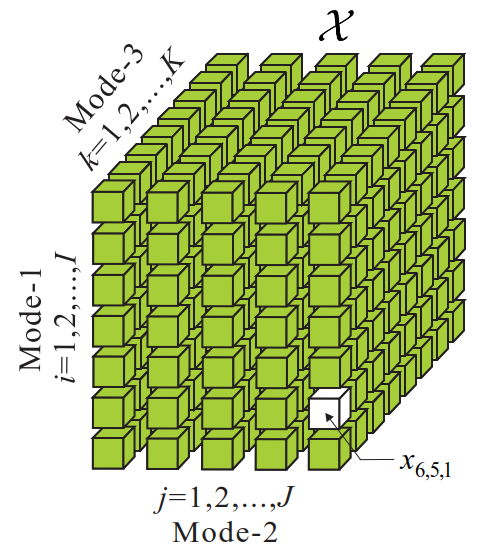
\includegraphics[height=0.7\paperheight]{figs/tensor_shape}
	\label{fig:tensor_shape}
\end{figure}
\end{frame}

\begin{frame}{What is tensor?}
\begin{figure}
	\centering  
	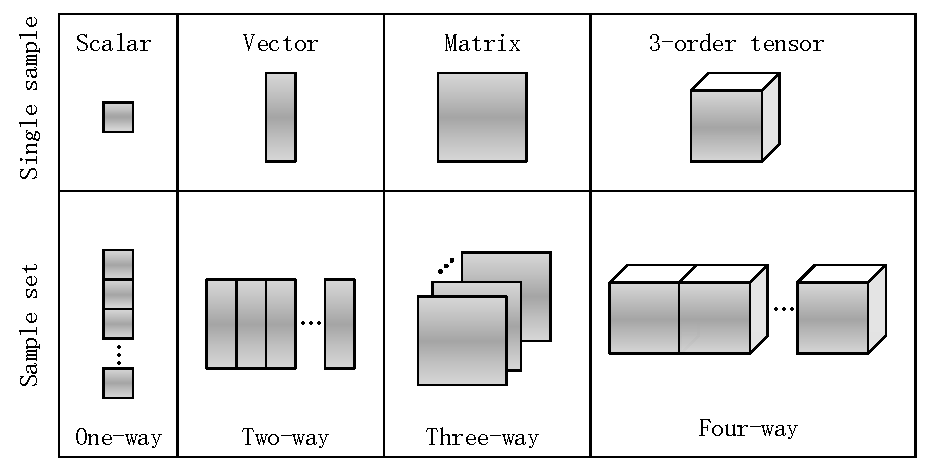
\includegraphics[height=0.7\paperheight]{figs/tensor_sample}
	\label{fig:tensor_sample}
\end{figure}
\end{frame}

\begin{frame}{Tensor fibers}
\begin{figure}
	\centering  
	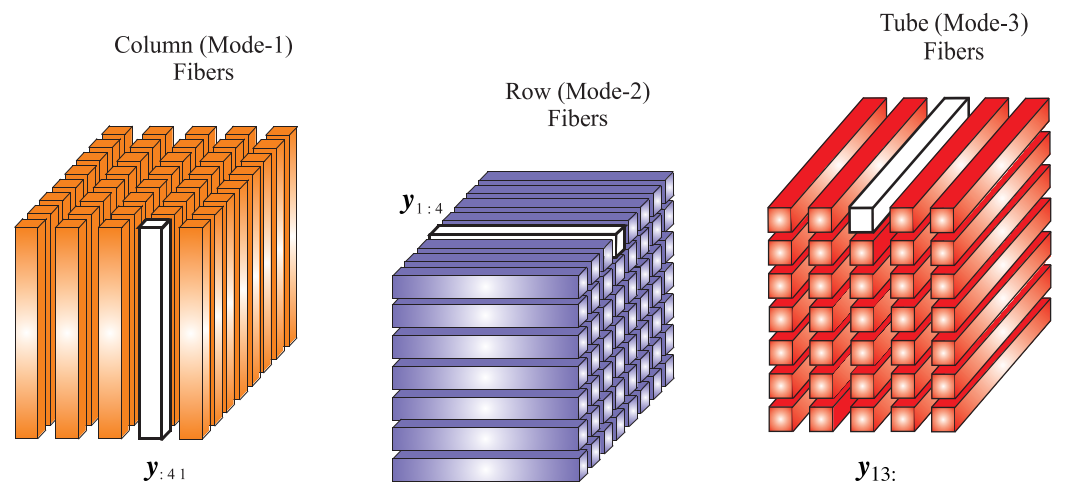
\includegraphics[width=\linewidth]{figs/tensor_fibers}
	\label{fig:tensor_fibers}
\end{figure}
\end{frame}

\begin{frame}{Tensor slices}
\begin{figure}
	\centering  
	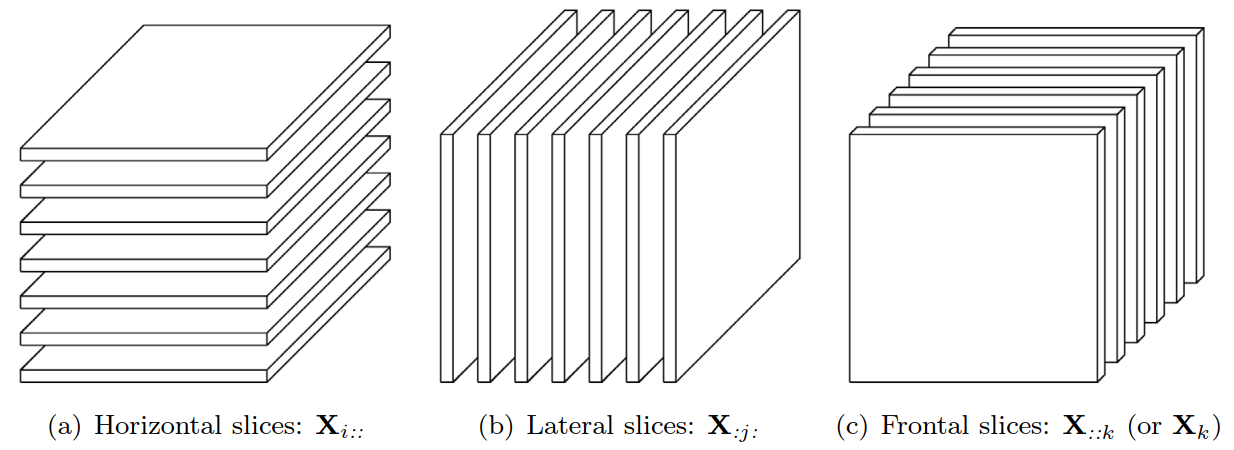
\includegraphics[width=\linewidth]{figs/tensor_slices}
	\label{fig:tensor_slices}
\end{figure}
\end{frame}

\begin{frame}{Agenda}
\begin{itemize}
    \large \item {Background}
    \large \item \textcolor{red}{Tensor Decompositions (CP, Tucker, and Tensor-Train)}
    \large \item{Transform-based Tensor Model and Applications}
    \large \item{Tensor Computations}
\end{itemize}
\end{frame}


\end{document}
